% make sure you have the VPN on, so that latex can load packages on the fly
% upload the project folder to overleaf

\documentclass{article}

% graphics package
\usepackage{graphicx} 

% enhanced citation package 
\usepackage{natbib}
\bibpunct{(}{)}{;}{a}{}{,}  % to adjust punctuation in references


% adjust caption properties
\usepackage[margin=10pt, font=small, labelfont=bf]{caption} 

% hyperrefs on, with nicer colors
\usepackage{color}
\usepackage{xcolor}
\usepackage[]{hyperref}
\definecolor{darkblue}{rgb}{0,0,.5}
\hypersetup{colorlinks=true, breaklinks=true, linkcolor=darkblue, menucolor=darkblue, urlcolor=darkblue, citecolor=darkblue}

% enhanced tables
\usepackage{multicol}              
\usepackage{multirow}
\usepackage{booktabs}  


\author{Your name(s)}
\title{Title of your paper}

\begin{document}
\maketitle

\begin{abstract}
Follow the instructions in the lecture notes concerning scientific writing. 
\end{abstract}

\section{Introduction}
Use references in yourbibtexfile, e.g. \citep{Farrell-Cheaptalk-1996}.

\section{Methods}
...

\section{Results}
Present your results here, use your produced figures. Refer to your figures and explain what we see in fig. \ref{myplot}

\begin{figure}
	\centering
	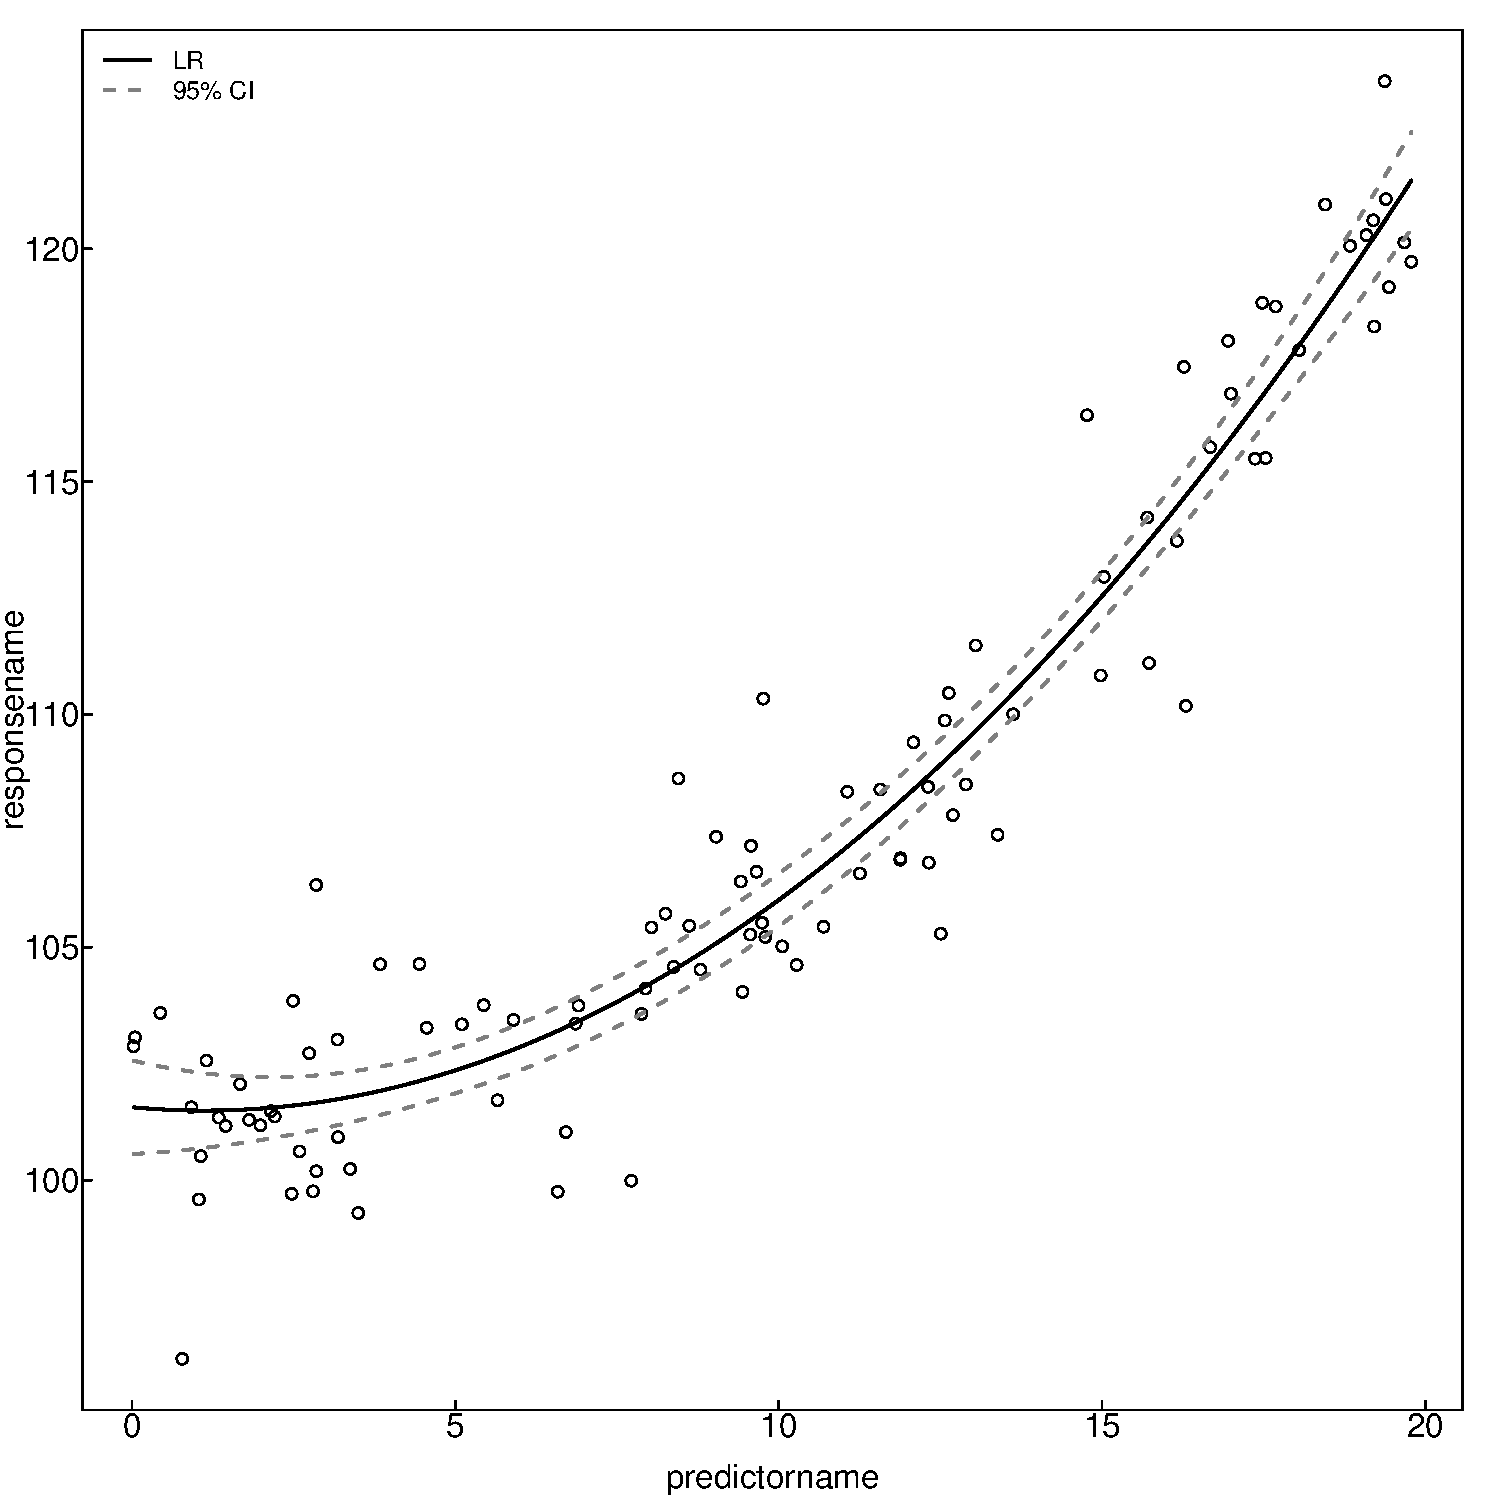
\includegraphics[width = 0.6\textwidth]{03-data/results/myplot.pdf}
	\caption{explain what to see. \label{myplot}}
\end{figure}

\section{Discussion}
...


% this is the style file. If you need to change something, google if the file you need is already there. If not (very uncommon) google makebst.
\bibliographystyle{chicago} 

% this is the bibtex libary file.
\bibliography{01-literature/yourbibtexfile}

% Note: all files can be anywhere, just give the full path.


\end{document}
